\documentclass[12pt,fleqn]{article}\usepackage{../../common}
\begin{document}
Binom İçin Normal Yaklaşıksallığı

Merkezi Limit Teorisinden $\bar{X}$'nin her $X_i$ için aynı olan nüfus
beklentisi ve sapmasını içeren $N(\mu,\sigma)$ olarak dağılacağını
biliyoruz. Ve bu durum, nüfus {\em hangi dağılıma sahip olursa olsun}
geçerlidir. $X_1,..,X_n$ birbirinden bağımsız ve aynı Bernoulli olarak
dağılmış, ve onların toplamını temsil eden binom dağılımı $X$ olarak
tanımlayalım, o zaman

$$ X = X_1 + X_2 + .. +  X_n $$

Daha önceden biliyoruz ki $E(X_i) = p, Var(X_i) = p(1-p)$, standart sapma
varyansın karekökü. O zaman Merkezi Limit Teorisine göre, 

$$ 
Z = 
\frac{X/n - p}{\sqrt{p(1-p)/n}} =
\frac{X - np}{\sqrt{np(1-p)}}
$$

Soru

Amerikalıların yüzde 12'sinin zenci olduğunu biliyoruz. Eğer 1500 kişiyi
içeren bir örneklem alsaydık, bu örneklemde 170'den daha az zenci
olmasının olasılığı nedir? 

Cevap

\%12 nüfus parametresidir, yani $p=0.12$. Örneklem $n=1500$. Normal
yaklaşıksallaması ile 

\begin{minted}[fontsize=\footnotesize]{python}
from scipy.stats import norm
n = 1500
p = 0.12
mu = n*p
std = np.sqrt(n*p*(1-p))
print mu,std
print 'olasilik',norm.cdf(170,loc=mu,scale=std)
\end{minted}

\begin{verbatim}
180.0 12.585706178
olasilik 0.213437028747
\end{verbatim}

Yani $N(180,12.58)$ dağılımını elde ettik ve hesapları onun üzerinden
yaptık. Sonuç diyor ki verilen örneklem ve nüfus $p$ değeri ile 170 altında
zenci sayısı elde etmek oldukça düşük bir ihtimalde. 

Örnek

Diyelim ki elimizde bir Web sitesinin günlük ziyaret, tıklama sayılarını
gösteren bir veri seti var, CVR ziyaretçilerin sitedeki tıklayan müşteriye
dönüşmesi oranı (conversion). 

\begin{minted}[fontsize=\footnotesize]{python}
import pandas as pd
from scipy import stats
a = pd.DataFrame({'tiklama': [20.,2.,40.,5.,10.,100.],
                  'ziyaret': [100.,10.,300.,400.,30.,800.]})
a['cvr'] = a['tiklama'] / a['ziyaret'] 
print a
\end{minted}

\begin{verbatim}
   tiklama  ziyaret       cvr
0       20      100  0.200000
1        2       10  0.200000
2       40      300  0.133333
3        5      400  0.012500
4       10       30  0.333333
5      100      800  0.125000
\end{verbatim}

Bu veri seti için cvr'in 0.16, yani yüzde 16 olduğunu önceden biliyoruz. Üstteki
başarı oranı binom dağılı ile modellenebilir, ziyaretler "deneylerdir", yani
örneklem büyüklüğünü gösterirler. Tıklama ise başarıdır, önceki binom
örneğindeki aynı formülü kullanırsak, normal yaklaşıksallığı üzerinden bir
z-skoru hesaplayabiliriz,

\begin{minted}[fontsize=\footnotesize]{python}
p = 0.16
btest = lambda x: (x['cvr']-p) / np.sqrt( p*(1-p)/x['ziyaret'])
a['guven'] = a.apply(btest, axis=1)
a['guven'] = np.round(stats.zprob(a['guven'])*100,2)
print a
\end{minted}

\begin{verbatim}
   tiklama  ziyaret       cvr  guven
0       20      100  0.200000  86.24
1        2       10  0.200000  63.50
2       40      300  0.133333  10.39
3        5      400  0.012500   0.00
4       10       30  0.333333  99.52
5      100      800  0.125000   0.35
\end{verbatim}

Soru 

Amerika'da 2009 yılında halkın ne kadarının arabalarında yakıt tasarrufunu
desteklediği merak konusuydu. Bir Gallup telefon anketinde bu soru 1012
yetişkine (18 ve üstü yaşta) soruldu. Cevap 810 kişinin tasarrufu
desteklediği yönündeydi. Yani $n=1012,k=810$. O zaman $p$ için \%95 güven
aralığını bulun.

Cevap 

$$ \bigg(
\frac{810}{1012}
-1.96 \sqrt{ \frac{(810/1012)(1-810/1012)}{1012} } ,
1.96  \sqrt{ \frac{(810/1012)(1-810/1012)}{1012} }
\bigg)
$$

$$ = (0.776,0825) $$

Python ile

\begin{minted}[fontsize=\footnotesize]{python}
m = 810/1012.
low = m - 1.96*np.sqrt(m*(1-m)/1012.)
high = m + 1.96*np.sqrt(m*(1-m)/1012.)
print low, high
\end{minted}

\begin{verbatim}
0.775768711331 0.825021802503
\end{verbatim}

Soru

Borsa konusunda okuyuculara tiyo veren bir gazete, bir şirket hissesinin
belli bir olay ardından çoğunlukla yükseldiğini söylüyor. Yazara göre hisse
9 olay içinden 6'sında bu çıkmış. Buradan hareketle yazar hissenin tekrar
çıkma şansının 6/9=\%66.7 olduğunu iddia ediyor. Okuyucu bunu ciddiye alsın
mı?


Cevap 

Ufak örneklemler için Agresti ve Coull yöntemini kullanmak iyi olur, bu
yönteme göre başarılı olay sayısına iki, tüm olay sayısına 4 ekleriz (yani
2 başarısızlık eklemiş oluruz) ve $\hat{p} = (x+2)(n+4)$ elde edilir. Bu
ekler hem genel teorik olarak bir değişim yaratmaz, hem de örneklem
sayısını arttırarak Normal yaklaşıksallığını kullanabilmemizi sağlar. Güven
aralığı, 

\begin{minted}[fontsize=\footnotesize]{python}
x=6.;n=9.;p=(x+2)/(n+4); z = 1.96
print p + np.array([-1,+1])*z*np.sqrt(p*(1-p)/n)
\end{minted}

\begin{verbatim}
[ 0.29753517  0.93323406]
\end{verbatim}

Demek ki yazar okuyucularına kötü bir tavsiye vermiş, güven aralığının alt
kısmı \%30 olduğuna göre hissenin yükselmesi garanti değildir, garanti için
güven aralığının iki ucu da \%50 üzerinde olmalıydı. Noktasal tahmin
bağlamında \%66.7 rakamı da yanıltıcıdir. Bu yazar okuyucularının para
kaybetmesine sebep olabilir.

Örneklem Büyüklüğü

Bir araştırmacı $n$ bağımsız deney baz alınarak elde edilen binom
parametresi $p$'yi tahmin etmek istiyor, fakat kaç tane $n$ kullanması
gerektiğini bilmiyor. Tabii ki daha büyük $n$ değerleri daha iyi sonuçlar
verecektir, ama her deneyin bir masrafı vardır. Bu iki gereklilik nasıl
birbiri ile uzlaştırılır?

Yeterli olacak en az kesinliği, duyarlılığı (precision) bulmak için Z
transformasyonu kullanılabilir belki. Diyelim ki $p$ için maksimum olurluk
tahmini olan $X/n$'in en azından $100(1-\alpha)\%$ olasılıkta $p$'nin $d$
kadar yakınında olmasını istiyoruz. O zaman alttaki denklemi tatmin eden en
ufak $n$'i bulduğumuz anda problemimizi çözdük demektir, 

$$ P\bigg( -d \le \frac{X}{n} - p \le d \bigg)  = 1-\alpha
\mlabel{1}
$$

Tahmin edici $X/n$'nin kendisi de bir rasgele değişkendir. Bu değişken
normal olarak dağılmıştır, çünkü $X$ Binom olarak dağılmış ise, bu dağılım
ayrı Bernoulli dağılımlarının toplamına eşittir. Fakat başka bir irdeleme
bizi daha basitçe sonuca götürür, binom dağılımı bir toplamdır, bu toplamı,
yani $X$'i $n$ ile bölüyorsak, otomatik olarak bir aritmetik averaj işlemi
yapmış oluyoruz. Bağımsız özdeşçe dağılmış (ıid) rasgele değişkenlerin
aritmetik ortalaması Merkezi Limit Kanunu'na göre normal'e yaklaştığına
göre o zaman, elimizde bir normal dağılım var demektir.

Standardize etmek için $X/n$'den beklentiyi çıkartıp standart sapmaya
bölebiliriz. Beklenti zaten çıkartılmış durumda (şansa bak!),
beklentinin ne olduğunu kontrol edelim tabii, ezbere yapmayalım bu işi,
eğer her Bernoulli'yi $X_i$ olarak temsil edersek,

$$ X = X_1 + .. + X_n $$

$$ X/n = 1/n(X_1 + .. + X_n )$$

$$ E[X/n] = E[1/n(X_1 + .. + X_n )]$$

$$  = 1/nE[(X_1 + .. + X_n )]$$

$$  = (1/n)np = p$$

Varyans için

$$
Var(X/n) = \frac{1}{n^2}Var(X) = \frac{1}{n^2}np(1-p)=
\frac{1}{n}p(1-p) 
$$

Binom dağılımlar için $Var(X) = np(1-p)$ olduğunu biliyoruz. Standart sapma
üstteki ifadenin karekökü, yani

$$ Std(X/n) = \sqrt{p(1-p)/n}
$$

Simdi standardize edelim,

$$ P\bigg( 
\frac{-d}{\sqrt{p(1-p)/n}} \le 
\frac{\frac{X}{n} - p }{\sqrt{p(1-p)/n}}\le 
\frac{d}{\sqrt{p(1-p)/n}} 
\bigg)  = 
1-\alpha$$


$$ P\bigg( 
\frac{-d}{\sqrt{p(1-p)/n}} \le 
Z
\frac{d}{\sqrt{p(1-p)/n}} 
\bigg)  = 
1-\alpha$$

Daha önceki z-skoru içeren eşitsizlikleri hatırlarsak, üstteki ifade 

$$ \frac{d}{\sqrt{p(1-p)/n}} = z_{\alpha/2} 
$$

O zaman 

$$ \frac{z_{\alpha/2}^2p(1-p)}{d^2} = n $$

Fakat bu bir nihai sonuç olamaz, çünkü $n$, $p$'nin bir fonksiyonun haline
geldi ve $p$ bilinmeyen bir değer. Fakat biliyoruz ki $0 \le p \le 1$, ve
$p(1-p) \le \frac{1}{4}$. Yani bir üst sınır (upper bound) elde ettik. 

Bunu kontrol edelim, $p(1-p)$ hangi $p$'de maksimize olur? $p$'ye göre
türev alırız, sıfıra eşitleriz, $(p-p^2)' = 1 - 2p = 0, p=1/2$. Ve hesabı
yaparsak, $1/2(1-1/2)=1/4$. Demek ki $p(1-p)$ değeri $1/4$'ten daha büyük
olamaz. Buna göre, üstteki formüle $p(1-p)$ yerine onun olabileceği en
büyük değeri koyarsak, 

$$ \frac{z_{\alpha/2}^21/4}{d^2} = n $$

$$ n = \frac{z_{\alpha/2}^2}{4d^2} $$

Not: $p(1-p)$, 1/4 değerinden daha küçük olabilir mi? Olabilir. Bu durumda
$n$ üstteki formülden elde edebileceğimiz değerden daha küçük te
çıkabilecektir. Fakat $p(1-p)$'in olabileceği en büyük değer 1/4'u
kullanarak ``$n$'in bundan daha büyük olmasına gerek yok'' diyebilen bir
formüle erişmiş olduk, yani, aslında $n$ için bir üst sınır elde ettik. 

Örnek

Büyük bir şehirde çocukların kaçta kaçının aşısını almış olup olmadığını
anlamak için bir anket gerçekleştirilecek. Anketi düzenleyenler örneklem
oranı olan $X/n$'in en az 98\% oranda gerçek oran $p$'nin 0.05 yakınında
olmasını istiyorlar. Örneklem ne kadar büyük olmalıdır? 

Burada $100(1-\alpha) = 98$, o zaman $\alpha = 0.02$, demek ki $z_{\alpha/2}
= z_{0.02/2} = z_{0.01}$ değerine ihtiyacımız var. Python ile

\begin{minted}[fontsize=\footnotesize]{python}
from scipy.stats.distributions import norm
print norm.ppf(0.99)
\end{minted}

\begin{verbatim}
2.32634787404
\end{verbatim}

Tüm hesap için

$$ n = \frac{(2.33)^2}{4(0.05)^2} = 543$$

Demek ki kabul edilebilir en ufak değer 543. 

Hata Payı (Margin of Error)

Basında oranları rapor ederken onunla beraber telafuz edilen bir kavram
hata payıdır. Aslında bu binom dağılımlarda güven aralığı ile çok yakından
alakalıdır;  hata payı \%95 güven aralığının en maksimum genişliğinin yarısı
olarak bilinir. Yani \%95 aralığının bir ucunu diğer ucundan çıkartırsak ve
ikiye bölersek, istenen sonuca erişiriz. Formülsel olarak genişlik $w$,

$$ w = \frac{k}{n} + 
1.96 \sqrt{\frac{(k/n)(1-k/n)}{n}} - 
- \bigg[ 
\frac{k}{n} -
1.96 \sqrt{\frac{(k/n)(1-k/n)}{n}}
\bigg]
 $$

$$ = 3.92 \sqrt{\frac{(k/n)(1-k/n)}{n}} $$

Şimdi $(k/n)(1-k/n)$ çarpımını düşünelim. [8] bölümünde gördük, $n$ her
zaman $k$'den büyük olduğuna göre $k/n$ her zaman 0 ve 1 arasındadır, o
zaman $(k/n)(1-k/n) \le 1/4$ olmalıdır, yani gösterilen çarpım 1/4'ten
büyük olamaz. Bunu alıp üstteki formül içine koyarsak,

$$ \max w = 3.92 \sqrt{\frac{1}{4n}} $$

elde ederiz. Bunun yarısı hata payıdır $d$ olur, yani

$$ d = \frac{0.98}{\sqrt{n}} $$

Örnek

Bir seçim kampanyası sırasında A ve B adayları arasında hangisinin daha
önce olduğunu bulmak için bir anket yapılır. Telefonda 597 kişiye
sorulduğunda A adayının 299 kişinin oyunu alacağı saptanmıştır. Basın
durumu ``A adayının avantajı hata payı \%4 içinde olduğu için o önde kabul
edilebilir'' diye rapor etmiştir. A oylarının hata payı hakikaten
\%4'müdür?

\begin{minted}[fontsize=\footnotesize]{python}
n = 597.
k = 299
print n/2
print k/n
d = 0.98/np.sqrt(n) 
print d*100
\end{minted}

\begin{verbatim}
298.5
0.500837520938
4.01087299444
\end{verbatim}

Evet hata payı \%4 çıktı. 

Dikkat edilirse hata payının anketten gelen sonuçlarla hiçbir alakası yok,
A için tercih \%25, \%75 olabilirdi ama üstteki hata payı hesabı yine aynı
kalırdı. Bunun sebebi formülün $n$'ye bağlı olması. 

Daha önemli soru hata payı basının üstteki ifadesinin gerçekten seçim
sonucu ile alakalı olup olmadığı! 

Hipotez Testleri (Hypothesis Testing)

İstatistik tek ya da aralıklar olarak sayısal tahminler üretmenin ötesinde,
``iki şey arasında birisini seçmek'' türünde bir karar bağlamında da
kullanılabilir. Bir psikolog bir davaya uzman görüş vermek için
çağrılmıştır ve sanık hakkında 'aklı olarak dengesiz ya da dengeli'
arasında bir seçim yapacaktır. İlaç regülasyonu ile uğraşan kurum yeni bir
ilaç hakkında 'etkili' ya da 'etkisiz' şeklinde bir karara ulaşacaktır. 

Bir deneyin mümkün sonuçlarını belli seçeneklere yönlendirip olasılık
teorisini kullanarak bunlardan birisini seçmeye İstatistik biliminde
Hipotez Test Etmek adı verilir.  

Birbiriyle yarış halinde olan iki hipotez vardır, bunlar sıfır hipotezi
($H_0$ olarak yazılıyor) ve alternatif hipotezdir ($H_1$ olarak
yazılıyor). $H_o$ ve $H_1$ arasında nasıl seçim yapacağımız kavramsal
olarak bir davada jürinin yaptığı seçime benzer: aynen sanığın, tersi
ispatlanana kadar, masum kabul edilmesi gibi eğer veri tersi sonuca varmaya
yetmezse $H_0$ da ``kabul edilir'', yani suçsuzluğun devam etmesi gibi
$H_0$ görüşü terkedilmemiş olur. Statüko devam eder. Bu kararı verirken
mahkemenin kanıtları incelemesi, hipotez testinde rasgele değişkenlerle
verinin üzerinden hesaplar yapmaya benzer.

Bunu bir örnek üzerinden daha iyi anlayabiliriz. Diyelim ki araba üreten
bir şirket yakıt performansını (gas mileage) arttırmaya uğraşıyor. Benzine
katılan yeni bir madde üzerinde deneyler yapıyorlar, deney için Boston /
Los Angeles arasında 30 tane araba sefer yapıyor. Yeni katkı maddesi
olmadığı durumda (statüko) yakıt performansının ortalama 25.0 mil/galon ve
standart sapmanın 2.4 mil/galon olduğu biliniyor. Diyelim ki deney
sonrasında arabalar ortalama olarak $\bar{y}$=26.3 mil/galon performansı
göstermişler. Katkı maddesi etkili mi, etkili değil mi?

Araştırmacılar 25.0'dan 26.3'e olan değişikliği daha önce bahsettiğimiz
mahkeme örneğindeki gibi bir çerçevede incelerler. Tipik olarak sıfır
hipotezi statükoyu temsil eder, yani değişmesi için ``ezici şekilde aksi
yönde veri olması gereken şey'' budur. Öyle değil mi? Eğer etkisiz bir
katkı maddesine evet dersek, ve ileride öyle olmadığı belli olursa bunun
şirket için çok negatif etkileri olacaktır, aynen masum bir kişiyi
yanlışlıkla hapse atmış olmak gibi. O yüzden kalmak istediğimiz güvenli
konum $H_0$'i temsil etmelidir. 

Bu noktada problemi rasgele değişkenlerin terminolojisi üzerinden tekrar
tanımlamak faydalı olur. Diyelim ki test sırasında 30 tane aldığımız ölçüm
$y_1,..,y_n$, her $y_i$ normal olarak dağılmış ve bu dağılımların $\mu$'şu
aynı, ve $\mu$'u birazdan ``eski'' ölçümlerin ortalaması olarak alacağız,
çünkü çürütmek istediğimiz hipotez bu. Ayrıca daha önceki tecrübelerimiz
gösteriyor ki $\sigma = 2.4$. Yani,

$$ 
f_Y(y;\mu) = \frac{1}{\sqrt{2\pi}(2.4)} 
e^{-\frac{1}{2}(\frac{y-\mu}{2.4})^2},
-\infty < y < \infty
$$

Hipotezleri şöyle tanımlayalım,

$H_0$: $\mu = 25.0$ (Katkı maddesi etkili {\em değildir})

$H_0$: $\mu > 25.0$ (Katkı maddesi etkilidir)

Şimdi yeni dağılımı standardize edip, bir hayali ortalama eşik değeri
üzerinden bir sonuç çıkartalım, standardize etmek için kullandığımız $\mu =
25.0$ çünkü eski ortalama bu. Şimdi diyelim ki test ettiğimiz eşik değer 25.25
(esas  amaç 26.3 ama oraya geleceğiz), aradığımız olasılık,

$$ P(\bar{Y}  \ge 25.25) $$

Üstteki ifade ``eğer örneklem eski dağılımdan geliyor olsaydı, 25.25
eşik değerini geçmesi ne kadar mümkün olabilirdi'' diye bir soru
soruyor. $\bar{Y}$'yi standardize edelim, o sırada eşitsizliğin sağ tarafı da
değişir,

$$ P(\frac{\bar{Y} - 25.0}{2.4 / \sqrt{30}} \ge 
\frac{25.25 - 25.0}{2.4 / \sqrt{30}}) 
$$


$$ P(Z \ge 0.57)$$

z-Skoru tablosunu kullanakarak bu hesabı yapmak için

$$ 1 - P(Z < 0.57)$$

0.57'nin z-skoru (satır 0.5 kolon .07) 0.7157 olarak gösterilmiş, o zaman
1-0.7157 = 0.2843. Kod ile

\begin{minted}[fontsize=\footnotesize]{python}
print 1-norm.cdf(0.57)
\end{minted}

\begin{verbatim}
0.284338849046
\end{verbatim}

Demek ki

$$ P(Z \ge 0.57) = 0.2843$$

Demek ki yeni deney sonuçlarının, eski dağılıma göre, eşik değerinden fazla
gelmesi hala az da muhtemel, demek ki eski hipotezi tam
çürütemedik. Seçtiğimiz eşik değeri bize kesin bir sonuç sağlamadı,
sezgisel olarak bu olasılığın büyük olduğunu görüyoruz. Mahkeme durumunda
suçsuz olması çok muhtemeldir diyemiyoruz. Ya da araba örneğinde (ve
pozitif bağlamda) yeni yakıt kesinlikle farklıdır / fazladır
diyemiyoruz. Bize daha kesin noktalar lazım, aklımızda bize ``acaba?''
dedittirecek eşik değerler istemiyoruz.

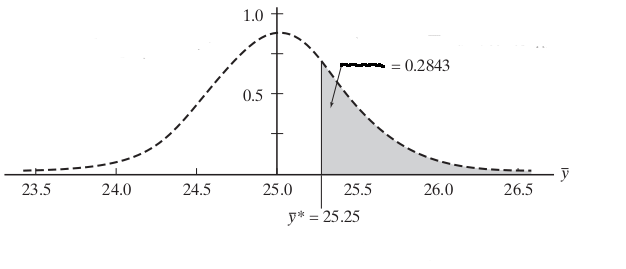
\includegraphics[height=6cm]{carhyp1.png}

Hayali eşik noktası $\bar{y}^\ast$'nin daha büyük yapsak (ki o zaman ona bağlı
olan sağdaki olasılık küçülecek). Bu olur mu? Eğer $\bar{y}^\ast = 26.50$
olsaydı? 

$$ P(\frac{\bar{Y} - 25.0}{2.4 / \sqrt{30}} \ge 
\frac{26.50 - 25.0}{2.4 / \sqrt{30}}) 
$$

$$ P(Z \ge 3.42) $$

$$ = 0.0003 $$

Bu olasılık ise çok küçük, yani eşik değeri çok büyük! Çıtayı çok fazla
kaldırdık, mahkeme durumunda sanki diyoruz ki suçun 1000 tane tanığı lazım,
sanık suçunu itiraf etmiş olmalı, herşey apaçık olmalı, bir de herşeyi
bizzat ben görmüş olmalıyım, yoksa kabul etmem. Araba örneğinde katkı
maddesi arabaya Formula-1 yarısı kazandırmazsa biz bu yakıtı daha iyi
olarak kabul etmeyiz diyoruz.

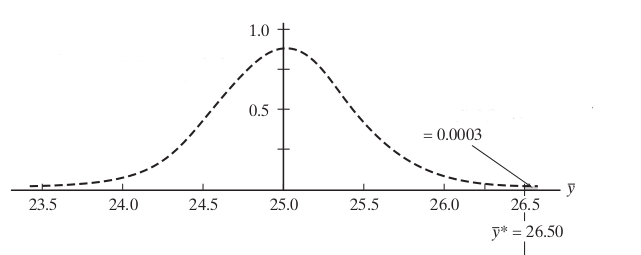
\includegraphics[height=6cm]{carhyp2.png}

Peki eğer 0.28 çok fazla, 0.0003 çok küçük ise hangi olasılık en iyi eşik
değerini verir? Bu soruya kesin olarak ve matematiksel bir cevap vermek
mümkün değil, fakat hipotez test etme tekniğini kullanan araştırmacıların
ulaştığı konsensüs 0.05 olasılık seviyesinin en iyi sonuçlar verdiğidir. Bu
durumda sıfır hipotezinin çok kolayca kenara atılmaması, ya da ona
gereğinden fazla bağlı kalınmaması mümkün oluyor.

O zaman 0.05 olasılığını verdirtecek eşik değeri hesaplayalım,

$$ P(\frac{\bar{Y} - 25.0}{2.4 / \sqrt{30}} \ge 
\frac{\bar{y}^\ast - 25.0}{2.4 / \sqrt{30}}) = 0.05
$$

$$ P(Z \ge  \frac{\bar{y}^\ast - 25.0}{2.4 / \sqrt{30}}) = 0.05
$$
ya da

$$ P(Z \le  \frac{\bar{y}^\ast - 25.0}{2.4 / \sqrt{30}}) = 0.95 $$

z-Skor tablosuna bakıyoruz, ``hangi z değeri 0.95 değeri sonucunu verir'',
kordinatlardan 1.64 z-skorunu buluyoruz. Ya da

\begin{minted}[fontsize=\footnotesize]{python}
print norm.ppf(0.95)
\end{minted}

\begin{verbatim}
1.64485362695
\end{verbatim}


$$ P(Z \le 1.64)  = 0.95 $$
O zaman 

$$ \frac{\bar{y}^\ast - 25.0}{2.4 / \sqrt{30}} = 1.64 $$

ve buradan $\bar{y}^\ast = 25.178$ sonucu çıkıyor. 26.3 değeri bu değerden
yüksektir demek ki sıfır hipotezi çürütülmüştür. Yeni yakıt katkısının
performansı arttırıyor olması büyük bir olasılıktır. 

Not: Bu testi aslında daha basit şekilde $\bar{y}^\ast = 26.3$ değerini
vererek elde edilen değeri 0.05'ten küçük olup olmadığına bakarak ta
yapabilirdik. Fakat metotu inşa ediyorduk o sebeple daha fazla örnekli
anlatmak gerekti. 

Örnek

SAT-I testinde ülke averajına oldukça yakın sonuçlar alan bir lisede yeni
bir müfredat denenmesine karar veriliyor. Deneme için 86 öğrenci rasgele
şekilde seçiliyor ve yeni bir tür cebir ve geometri dersine
sokuluyor. Sonraki SAT-1 testinde sonuçlarına göre bu çocuklar ortalama 502
sonuç almışlar, ülke çapındaki ortalama 494, standart sapma
124. $\alpha=0.05$ önemliliği (significance) seviyesinde yeni müfredatın
başarılı olduğu iddia edilebilir mi? 

İlk önce $\mu$ parametresinin yeni müfredatın gerçek ortalaması olduğunu
farzediyoruz. O zaman statüko nedir? Bu ortalamanın ülke ortalaması
seviyesinde kalmasıdır, yani $\mu_0 = 494$ olmasıdır. Fakat bu sefer
alternatif hipotez iki yönlü (two-sided) olmalı çünkü yeni müfredat, hiç
istenmese de, test sonuçlarında negatif sonuca da yol açabilir! O zaman
$H_0$'i reddetmeliyiz eğer z istatistiği $\le -z_{0.025}$ ise (yani
-1.96'dan küçük ise), ya da $\ge z_{0.025}$ (yani 1.96'dan büyük ise). 

$$ z = \frac{502-494}{124\sqrt{86}} = 0.60$$

Sonuç 1.96'dan büyük değil. O zaman $H_0$'i, yani statükoyu
değiştiremedik. Elde edilen sonuçlar bir ilerlemedir fakat bu ilerlemenin şans
eseri olması da muhtemel.

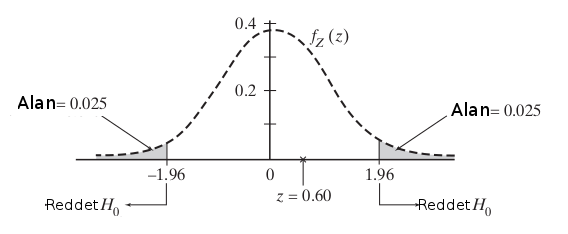
\includegraphics[height=5cm]{sat1.png}

Binom Hipotez Testleri

Örnek

Erteleme Teorisi: Yaygın bir inanışa göre insanlar ölüm tarihlerini onlar
için önemli bir gün sonrasına erteleyebiliyorlar, mesela kendi doğum
günleri, aile toplantıları, bir akrabanın dönüşünü beklemek, vs. gibi Hatta
ülke çapında seçimlerin bile ölüm günlerini etkilediği görülmüştür,
başkanlık seçimleri olan Eylül ve Ekim ayları sırasında ölüm oranlarının
düştüğü saptanmıştır. Bu teoriye göre pek çok yaşlı insan kimin kazandığını
görmek için ``biraz daha dayanıyor''.

Bir araştırma bu teorinin doğru olup olmadığını kontrol etti. Bu bağlamda
Salt Lake City şehrindeki bir gazetenin ölüm ilanı kısmına bakıldı ve 747
kişi içinden sadece 60 kişinin, daha doğrusu \%8'inin kendi doğumgünlerinin
3 ay öncesi içinde olduğunu saptadı. Eğer insanların ölümü rasgele olsaydı
yaklaşık olarak \%25'inin bu periyod içinde ölmesini beklerdiniz. O zaman
bu \%25'den \%8'e düşüşü nasıl açıklamalıyız?  Araştırma teoriyi
destekleyecek rakamları veriyor mu?

Diyelim ki 747 ölüm iki kategori üzerinden temsil edilsin, doğumgünü
öncesindeki 3 ay içinde ölenler ve ölmeyenler. $k_i=1$ ile $i$'inci kişinin
1. kategoriye, $k_i=0$ ise 2. kategoriye ait olmasını temsil ediyoruz. O
zaman $k = k_1 + k_2 + .. + k_{747}$ birinci kategorideki toplam ölümü
temsil ediyor. Üstteki her $k$ doğal olarak Binom dağılımı, ve $p$
parametresini kullanıyor ki 

$$ p = P(\textrm{sahıs doğumgünü öncesindeki 3 ay içinde ölüyor}) $$

Eğer insanlar ölümlerini ertelemeseydi $p = 3/12 = 0.25$ olurdu. Eğer
erteliyorlar ise $p$ 0.25'den daha küçük olmalı. Bu azalmanın ne kadar
önemli (significant) olduğunu irdelemek için tek taraflı bir Binom Testi
uygulamak lazım. 

$H_0$: $p = 0.25$

$H_1$: $p < 0.25$

Test için $p_0$ olduğunu farzettiğimiz ``gerçek'' dağılımı (ki statükoyu
onun üzerinden temsil edeceğiz) kullanacağız. 

$$ z = \frac{k-np_0}{\sqrt{np_0(1-p_0)}} \le -z_{0.05} = -1.64 $$

$$ = \frac{60-747(0.25)}{747(0.25)(0.75)} = -10.7 \le -1.64  $$

Test istatistiği kritik değerin aşırı derecede sol tarafına düştü. Demek ki
ezici miktarda kanıt, veri, sonuç elde ettik, \%25'ten \%8'e düşüşün pür
şans dışında başka bir sebebi var. Tabii bu sebep Erteleme Teorisi
haricinde bir şey de olabilir, fakat yine de ortaya çıkan kalıp bize ölüm
vaktimizin kontrolümüzde olduğunu destekleyen yönde bir sonuç veriyor.

Not: Üstteki test ``büyük örneklem'' olduğu durumlarda geçerlidir. Küçük
örneklem durumunda Binom dağılımının kendisi test için kullanılabilir.

Tek Örneklem t Testi (The One-Sample t test)

Bu test verinin bir $N(\mu,\sigma)$ Normal dağılımından geldiğini farzeder,
test etmek istediğimiz hipotez / karşılaştırma $\mu = \mu_0$. Ayrıca
$\sigma$ bilinmiyor, ki Öğrenci t dağılımından bahsetmemizin ana sebebi
buydu zaten, o zaman hipotez testine Tek Örneklem t Testi adı verilir.

Örnek

Alttaki veride bir grup hanımın ne kadar kalori tükettiği
kayıtlanmış. Acaba bu hanımların aldığı enerji tavsiye edilen 7725'ten ne
kadar sapmıştır?

\begin{minted}[fontsize=\footnotesize]{python}
daily_intake = np.array([5260.,5470.,5640.,6180.,6390.,6515.,6805.,\
7515.,7515.,8230.,8770.])
\end{minted}

Örneklem küçük. O sebeple t dağılımı kullanmak mantıklı. t değerini
$\frac{\bar{y}-\mu_o}{s/\sqrt{n}}$ olarak hesaplayacağız, ki $\mu_0=7725$
olacak.

\begin{minted}[fontsize=\footnotesize]{python}
from scipy.stats.distributions import t
import pandas as pd, math
data = pd.DataFrame(daily_intake)
n = len(data)
df = n-1 # serbestlik derecesi
mu0 = 7725.
ybar = float(data.mean())
s = float(data.std())
print 'ortalama',ybar,'std',s
tval = (ybar-mu0)/(s/np.sqrt(n))
print 'df',df,'tval',tval
print 'sol',t.ppf(0.025,df)
print 'sag',t.ppf(0.975,df)
\end{minted}

\begin{verbatim}
ortalama 6753.63636364 std 1142.12322214
df 10 tval -2.82075406083
sol -2.22813885196
sag 2.22813885196
\end{verbatim}

Sol ve sağ eşik değerlerini hesapladık ve t değeri bu aralığın içine
düşmüyor. Yani hipotezi reddediyoruz. Bazıları bu problemde p değeri görmek
isteyebilir, 

\begin{minted}[fontsize=\footnotesize]{python}
print 't degeri', tval
print 'iki tarafli p degeri', 2*t.cdf(tval,df)
\end{minted}

\begin{verbatim}
t degeri -2.82075406083
iki tarafli p degeri 0.0181372351761
\end{verbatim}

p değeri hesapladık 0.05'ten küçük çıktı. İkiyle çarpmamızın sebebi
iki-taraflı p-testi yapmış olmamız, yani kabul edilebilir bölgenin hem
solundan hem de sağından ne kadar dışına düşüyorsak, bu iki taraftaki p
değerini birbirine toplamalıyız. Tabii t dağılımı simetrik olduğu için her
iki taraftan da aynı şekilde dışarıda kalıyoruz. Bazı kaynaklar iki taraflı
p testinin $|t| < -t_{esik,derece}$ karşılaştırmasını yaptığını söyler.

Benzer bir hesabı kütüphane çağrısı ile yaparsak,

\begin{minted}[fontsize=\footnotesize]{python}
from scipy.stats import ttest_1samp
t_statistic, p_value = ttest_1samp(daily_intake, mu0)
print 't', t_statistic, 'one-sample t-test', p_value
\end{minted}

\begin{verbatim}
t -2.82075406083 one-sample t-test 0.0181372351761
\end{verbatim}

Sonuç p değeri 0.05'ten küçük çıktı yani yüzde 5 önemliliğini
(significance) baz aldık bu durumda veri hipotezden önemli derecede
(significantly) uzakta. Demek ki ortalamanın 7725 olduğu hipotezini
reddetmemiz gerekiyor.

İki Örneklemli Test

Gruplar 0/1 değerleri ile işaretlendi, ve test etmek istediğimiz iki grubun
ortalamasının (mean) aynı olduğu hipotezini test etmek. t-test bu arada
varyansın aynı olduğunu farzeder.

\begin{minted}[fontsize=\footnotesize]{python}
energ = np.array([
[9.21, 0],[7.53, 1],
[7.48, 1],[8.08, 1],
[8.09, 1],[10.15, 1],
[8.40, 1],[10.88, 1],
[6.13, 1],[7.90, 1],
[11.51, 0],[12.79, 0],
[7.05, 1],[11.85, 0],
[9.97, 0],[7.48, 1],
[8.79, 0],[9.69, 0],
[9.68, 0],[7.58, 1],
[9.19, 0],[8.11, 1]])
group1 = energ[energ[:, 1] == 0][:, 0]
group2 = energ[energ[:, 1] == 1][:, 0]
t_statistic, p_value = ttest_ind(group1, group2)
print "two-sample t-test", p_value
\end{minted}

\begin{verbatim}
two-sample t-test 0.00079899821117
\end{verbatim}

$p$ değeri $< 0.05$ yani iki grubun ortalaması aynı değildir. Aynı olduğu
hipotezi reddedildi.

Eşlemeli t-Test (Paired t-test)

Eşlemeli testler aynı deneysel birimin ölçümü alındığı zaman
kullanılabilir, yani ölçüm alınan aynı grupta, deney sonrası deneyin
etki edip etmediği test edilebilir. Bunun için aynı ölçüm deney
sonrası bir daha alınır ve "farkların ortalamasının sıfır olduğu"
hipotezi test edilebilir. Altta bir grup hastanın deney öncesi ve
sonrası ne kadar yiyecek tükettiği listelenmiş. 

\begin{minted}[fontsize=\footnotesize]{python}
intake = np.array([
[5260, 3910],[5470, 4220],
[5640, 3885],[6180, 5160],
[6390, 5645],[6515, 4680],
[6805, 5265],[7515, 5975],
[7515, 6790],[8230, 6900],
[8770, 7335],
])
pre = intake[:, 0]
post = intake[:, 1]
t_statistic, p_value = ttest_1samp(post - pre, 0)
print "paired t-test", p_value
\end{minted}

\begin{verbatim}
paired t-test 3.05902094293e-07
\end{verbatim}

Wilcoxon işaretli-sıralı testi (Wilcoxon signed-rank test)

t Testleri Normal dağılıma göre sapmaları yakalamak açısından,
özellikle büyük örneklemler var ise, oldukça sağlamdır. Fakat bazen
verinin Normal dağılımdan geldiği faraziyesini yapmak istemeyebiliriz.
Bu durumda {\em dağılımdan bağımsız metotlar} daha uygundur, bu tür
metotlar için verinin yerine çoğunlukla onun sıra istatistiklerini
(order statistics) kullanır.

Tek örneklemli Wilcoxon testi için prosedür $\mu_0$'i tüm veriden çıkartmak ve
geri kalan (farkları) işaretine bakmadan sayısal (numeric) değerine göre
sıralamak, ve bu sıra değerini bir kenara yazmak. Daha sonra geri dönüp bu sefer
çıkartma işlemi sonucunun işaretine bakmak, ve eksi işareti taşıyan sıra
değerlerini toplamak, aynı işlemi artı işareti için yapmak, ve eksi toplamı artı
toplamından çıkartmak. Sonuçta elimize bir istatistik $W$ gelecek. Bu test
istatistiği aslında $1..n$ tane sayı içinden herhangi birini $1/2$ olasılığıyla
seçmek, ve sonuçları toplamaya tekabül etmektedir. Ve bu sonuç yine \verb!0.05!
  ile karşılaştırılır.

\begin{minted}[fontsize=\footnotesize]{python}
from scipy.stats import wilcoxon, ttest_ind
daily_intake = np.array([5260,5470,5640,6180,6390,6515,6805,7515,7515,8230,8770])
z_statistic, p_value = wilcoxon(daily_intake - 7725)
print "one-sample wilcoxon-test", p_value
\end{minted}

\begin{verbatim}
one-sample wilcoxon-test 0.0279991628713
\end{verbatim}

Hipotezi reddettik.

Eşlemeli t-testi şimdi Wilcoxon testi ile yapalım,

\begin{minted}[fontsize=\footnotesize]{python}
z_statistic, p_value = wilcoxon(post - pre)
print "paired wilcoxon-test", p_value
\end{minted}

\begin{verbatim}
paired wilcoxon-test 0.00463608893545
\end{verbatim}

Normallik Testi

Paket \verb!scipy.stats! altında normallik testleri için bazı çağrılar var,
bu tekniklerden ikisini altta gösteriyoruz,

\begin{minted}[fontsize=\footnotesize]{python}
import scipy.stats as st
arr = np.array([3,4,3,10,10,444,444,3,98])
arr2 = np.array([np.random.normal() for i in range(100)])

print 'D-Agostino and Pearsons'
print st.normaltest(arr)
print st.normaltest(arr2)
print
print 'Shapiro-Wilk'
print st.shapiro(arr)
print st.shapiro(arr2)
\end{minted}

\begin{verbatim}
D-Agostino and Pearsons
(4.6919700569024814, 0.095752836393526289)
(1.4265636263795889, 0.49003335773235424)

Shapiro-Wilk
(0.6167718172073364, 0.00015052134403958917)
(0.9891485571861267, 0.5962899923324585)
\end{verbatim}

Sonuçlara göre Shapiro-Wilk yaklaşımı daha güvenilir gözüküyor, zaten [6,
sf 53]'e göre örneklem sayısı $\le 50$ olduğu durumlarda bu test tercih
edilmelidir.

Biraz Matematik

Diyelim ki Gaussian dağılımına sahip olduğunu düşündüğümüz $\{ x_i\}$
verilerimiz var. Bu verilerin Gaussian dağılımına uyup uymadığını nasıl
kontrol edeceğiz? Normal bir dağılımı her veri noktası için şöyle temsil
edebiliriz,

$$ y_i = \Phi\bigg(\frac{ x_i - \mu}{\sigma}\bigg) $$

Burada $\Phi$ standart Gaussian'ı temsil ediyor (detaylar için [7] ve CDF
fonksiyonuna tekabül ediyor. CDF fonksiyonunun aynı zamanda yüzdelik dilimi
(quantile) hesapladığı söylenir, aslında CDF son derece detaylı bir
olasılık değeri verir fakat evet, dolaylı yoldan noktanın hangi çeyrek
içine düştüğü de görülecektir.

Şimdi bir numara yapalım, iki tarafa ters Gaussian formülünü uygulayalım,
yani $\Phi^{-1}$.

$$ \Phi^{-1}(y_i) = \Phi^{-1}\bigg( \Phi\bigg(\frac{ x_i - \mu}{\sigma}\bigg)\bigg) $$

$$ \Phi^{-1}(y_i) = \frac{ x_i - \mu}{\sigma}$$

$$ x_i = \Phi^{-1}(y_i) \sigma + \mu  $$ 

Bu demektir ki elimizdeki verileri $\Phi^{-1}(y_i)$ bazında grafiklersek,
bu noktalar eğimi $\sigma$, kesisi (intercept, y ekseninin kesildiği yer)
$\mu$ olan bir düz çizgi olmalıdır. Eğer kabaca noktalar düz çizgi
oluşturmuyorsa, verimizin Gaussian dağılıma sahip olmadığına karar
verebiliriz.

Üstte tarif edilen grafik,  olasılık grafiği (probabılıty plot) olarak
bilinir. 

Ters Gaussian teorik fonksiyonunu burada vermeyeceğiz, Scipy
\verb!scipy.stats.ınvgauss! hesaplar için kullanılabilir. Fakat $y_i$'nin
kendisi nereden geliyor? Eğer $y_i$, CDF'in bir sonucu ise, pür veriye
bakarak bir CDF değeri de hesaplayabilmemiz gerekir. Bunu yapmak için bir
başka numara lazım. 

1. Eldeki sayıları artan şekilde sıralayın

2. Her veri noktasına bir derece (rank) atayın (sıralama sonrası hangi
seviyede olduğu yeterli, 1'den başlayarak). 

3. Çeyrek değeri $y_i$ bu sıra / $n+1$, $n$ eldeki verinin büyüklüğü. 

Bu teknik niye işliyor? $x$'in CDF'i $x_i < x$ şartına uyan $x_i$'lerin
oranı değil midir? Yani bir sıralama söz konusu ve üstteki teknik te bu
sıralamayı biz elle yapmış olduk, ve bu sıralamadan gereken bilgiyi aldık. 

Basit bir Gaussian kontrolü, \verb!qqplot! kullanarak. 

\begin{minted}[fontsize=\footnotesize]{python}
import statsmodels.api as sm
fig = sm.qqplot(arr)
plt.savefig('stat_tests_01.png')
\end{minted}
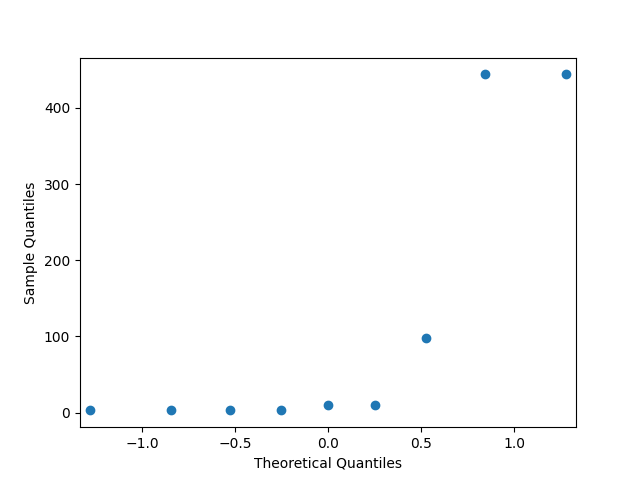
\includegraphics[height=6cm]{stat_tests_01.png}

Gerçekten Gaussian olan bir veri şöyle gözükür, 

\begin{minted}[fontsize=\footnotesize]{python}
fig = sm.qqplot(arr2)
plt.savefig('stat_tests_02.png')
\end{minted}
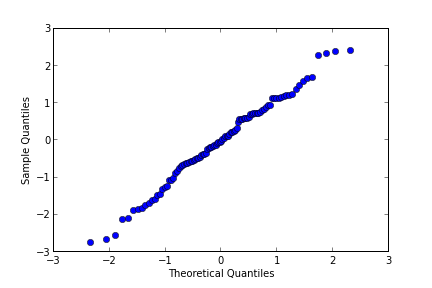
\includegraphics[height=6cm]{stat_tests_02.png}

Kaynaklar

[1] Dalgaard, {\em Introductory Statistics with R}

[2] Kerns, {\em Introduction to Probability and Statistics Using R}

[3] Blondel, {\em t-test and wilcoxon-test examples in Python}, url{https://gist.github.com/mblondel/1761714}

[4] Runger, {\em Applied Statistics and Probability for Engineers}

[5] Stack Exchange, {\em Sample variance converge almost surely}, \url{http://math.stackexchange.com/questions/243348/sample-variance-converge-almost-surely}

[6] Haslwanter, {\em Introduction to Statistics using Python}

[7] Bayramlı, İstatistik, {\em Giris})

[8] Bayramlı, Istatistik, {\em Örneklem Büyüklüğü}



\end{document}

